\documentclass[border=2mm]{standalone}
\usepackage{tikz}
\usetikzlibrary{shapes.geometric}

\begin{document}

\if09
diamond
    aspect
ellipse
trapezium
    trapezium left angle=45
    trapezium right angle=45
    trapezium angle=45
    trapezium stretches=
semicircle
regular polygon
    regular polygon sides=3
star
    star points=1
    star point height=0.5
    star point ratio=45
isosceles triangle
    isosceles triangle apex angle=45
    isosceles triangle stretches=true
kite
    kite upper vertex angle=45
    kite lower vertex angle=45
    kite vertex angles=45
dart
    dart tip angle=45
    dart tail angle=45
circular sector
    circular sector angle=
cylinder
    aspect=1
    cylinder uses custom fill
    cylinder end fill=red!50
    cylinder body fill=red!25
\fi


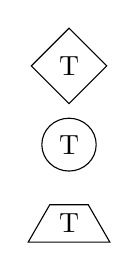
\begin{tikzpicture}[every node/.style={name=a,yshift=-1cm}]
    \path node[draw,diamond , aspect=1] at(0,0){T};
    \path node[draw,ellipse] at(a){T};
    \path node[draw,trapezium,trapezium stretches] at(a){T};
\end{tikzpicture}







 
 
\end{document}